{\begin{tikzpicture}[>=latex,scale=.5,baseline=10pt]
% Draw grid
\draw (-3,0)--(3,0);
\draw (0,-1)--(0,5);
\foreach \x in {-2,...,2}
 {\draw (\x,-.1)--(\x,.1);
 }
\foreach \x in {1,...,4}
 {\draw (-.1,\x)--(.1,\x);
 };
\node[below] at (1,-0.1) {1};
\node[left] at (0,1) {1};

\draw[->,thick] (0,0) -- (1,2) node [right] {\vx};
\draw[->,thick] (0,0) -- (-2,3) node [left] {\vy};
\end{tikzpicture}}
{Sketches will vary depending on choice of origin of each vector.

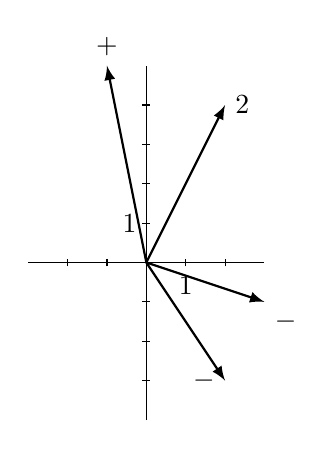
\begin{tikzpicture}[>=latex,scale=.5]
% Draw grid
\draw (-3,0)--(3,0);
\draw (0,-4)--(0,5);
\foreach \x in {-2,...,2}
 {\draw (\x,-.1)--(\x,.1);
 }
\foreach \x in {-3,...,4}
 {\draw (-.1,\x)--(.1,\x);
 };
\node[below] at (1,-0.1) {1};
\node[left] at (0,1) {1};

\draw[->,thick] (0,0) -- (2,4) node [right] {$2\vx$};
\draw[->,thick] (0,0) -- (2,-3) node [left] {$-\vy$};
\draw[->,thick] (0,0) -- (-1,5) node [above] {$\vx+\vy$};
\draw[->,thick] (0,0) -- (3,-1) node [below right] {$\vx-\vy$};

\end{tikzpicture}
}